%% Copyright 2015 M. Harland
  %
  % This work may be distributed and/or modified under the
  % conditions of the LaTeX Project Public License, either version 1.3
  % of this license or (at your option) any later version.
  % The latest version of this license is in
  %   http://www.latex-project.org/lppl.txt
  % and version 1.3 or later is part of all distributions of LaTeX
  % version 2005/12/01 or later.

%%%%%%%%%%
\documentclass[12pt,a4paper]{article}

\usepackage[left=2.5cm,right=2.5cm,top=1.0cm,bottom=2cm]{geometry}
\usepackage{placeins}

%\usepackage{graphicx}
%\usepackage{subcaption}
%\usepackage{amsmath}
%\parindent=1cm
%%%%%%%%%



%\marginparwidth = 0pt
%\hoffset = 0pt
%\oddsidemargin = 0pt
%\marginparsep = 0pt
%\voffset = 0pt

%\documentclass{amsproc}
%\documentclass[11pt,
%paper=a4,
%bibtotocnumbered,	  % Literaturverzeichnis ins Inhaltsverzeichnis
%liststotocnumbered,  % Alle Listen ins Inhaltsverzeichnis							
%DIV=calc,		  % führt die Satzspiegelberechnung neu aus
%oneside,		  % einseitiger Druck
%tablecaptionabove,	  % Tabellenüberschriften aktivieren
%BCOR=16mm,	  % Bindekorrektur
%headinclude,
%footinclude
%]{article}


%%%%
%\usepackage{fancyhdr}
%\usepackage{lipsum} % only for showing some sample text
%\fancyhf{} % clear all header and footers
%\renewcommand{\headrulewidth}{0pt} % remove the header rule
%\rfoot{\thepage}
%\pagestyle{fancy}
%\usepackage{indentfirst} % Красная строка
%%%%




\usepackage{amssymb}
\usepackage{amsmath}
\usepackage{graphicx}
\usepackage{color}
\def\x{{\bf x}}
\def\y{{\bf y}}
\newcommand{\XY}[1]{\textcolor{magenta}{X$\rightarrow$ Y: #1}}

\usepackage{mathrsfs,bbm}
\usepackage{comment}
\newcommand{\bm}[1]{\boldsymbol #1}
\newcommand{\lh}{\mbox{$\neg$}}
\newcommand{\rh}{\reflectbox{$\neg$}}
\usepackage{txfonts}
\DeclareSymbolFont{symbols}{OMS}{cmsy}{m}{n}
\DeclareSymbolFont{largesymbols}{OMX}{cmex}{m}{n}

%%%%%%%%%%%%%%%%%%%%%%%%%%%%%%%%%%%%%%%%%%%%%%%%
%Genaral math symbols
\newcommand{\TR}{\text{Tr}}
\newcommand{\BK}{{\bm k}}
\newcommand{\Vk}{{\bm k}}
\newcommand{\Ks}{{{\bm k}\sigma}}
\newcommand{\tb}{{\bar t}}
\newcommand{\myast}{{{}\hspace*{-0.1em}\ast\hspace*{-0.1em}{}}}
\newcommand{\mydagger}{{\dagger}}
\newcommand{\phdagger}{{\phantom{\dagger}\!}}
\newcommand{\bra}[1]{\langle{#1}|}
\newcommand{\ket}[1]{|{#1}\rangle}
\newcommand{\braket}[2]{\langle{#1}|{#2}\rangle}
\newcommand{\expval}[1]{\langle{#1}\rangle}
%%%%%%%%%%%%%%%%%%%%%%%%%%%%%%%%%%%%%%%%%%%%%%%%
%Contour calculus notation
\newcommand{\CS}{\mathcal{S}}
\newcommand{\ii}{^j}
\newcommand{\delC}{\delta_\CC}
\newcommand{\intC}{\int_\CC}
\newcommand{\tmin}{t_{\text{min}}}
\newcommand{\tmax}{t_{\text{max}}}
\newcommand{\CC}{\mathcal{C}}
\newcommand{\TC}{\mathcal{T}_{\CC}}
\newcommand{\gtrc}{\succ}
\newcommand{\lesc}{\prec}
%%%%%%%%%%%%%%%%%%%%%%%%%%%%%%%%%%%%%%%%%%%%%%%%
%Keldysh Green functions
\newcommand{\convz}{\ast}
\newcommand{\convi}{\bullet}
\newcommand{\convr}{\circ}
\newcommand{\ret}{{\text{R}}}
\newcommand{\adv}{{\text{A}}}
\newcommand{\mat}{{\text{\tiny M}}}
\newcommand{\tv}{{\makebox{$\neg$}}}
\newcommand{\vt}{{\reflectbox{$\neg$}}}
\newcommand{\les}{<}
\newcommand{\lar}{>}
%%%%%%%%%%%%%%%%%%%%%%%%%%%%%%%%%%%%%%%%%%%%%%%%
%misc
\newcommand{\ETAL}{{\em et al.}}
\newcommand{\Ucdyn}{{U_{\text{dyn}}}}
\newcommand{\sss}{_{\alpha\alpha'}}
\newcommand{\YY}{Y}
\newcommand{\KK}{K}
\newcommand{\pseudo}{\widetilde}
\newcommand{\cyles}{\prec}
\newcommand{\scell}{\text{scel}}
\newcommand{\pG}{\mathcal{G}}
%%%%%%%%%%%%%%%%%%%%%%%%%%%%%%%%%%%%%
%FK
\newcommand{\Gwnull}{Q}\newcommand{\Gweins}{R}
\newcommand{\gwnull}{q}\newcommand{\gweins}{r}
%%%%%%%%%%%%%%%%%%%%%%%%%%%%%%%%%%%%%
% for Mott Breakdown
\renewcommand{\dh}{dh}
\newcommand{\jd}{\Gamma_\text{\dh}}
\newcommand{\fth}{F_\text{th}}
\newcommand{\hopp}{{t^*}}
\renewcommand{\bar}{\overline}

%\input{defs}
\newcommand{\cis}{c_{i\sigma}}
\newcommand{\cisd}{c_{i\sigma}^\dagger}
\newcommand{\cs}{c_{\sigma}}
\newcommand{\csd}{c_{\sigma}^\dagger}
\newcommand{\cst}{c_{\sigma}(\tau)}
\newcommand{\csdtp}{c_{\sigma}^\dagger(\tau')}
\newcommand{\nup}{n_{\uparrow}}
\newcommand{\ndown}{n_{\downarrow}}
\newcommand{\nupt}{\nup(\tau)}
\newcommand{\ndownt}{\ndown(\tau)}
\newcommand{\nuptp}{\nup(\tau')}
\newcommand{\ndowntp}{\ndown(\tau')}
\newcommand{\nuptpp}{\nup(\tau'')}
\newcommand{\ndowntpp}{\ndown(\tau'')}
\newcommand{\nupti}{\nup(\tau_i)}
\newcommand{\nupta}{\nup(\tau_1)}
\newcommand{\ndownti}{\ndown(\tau_i)}
\newcommand{\ndownta}{\ndown(\tau_1)}
\newcommand{\nuptj}{\nup(\tau_j)}
\newcommand{\nuptb}{\nup(\tau_2)}
\newcommand{\ndowntj}{\ndown(\tau_j)}
\newcommand{\ndowntb}{\ndown(\tau_2)}
\newcommand{\nuptk}{\nup(\tau_k)}
\newcommand{\ndowntk}{\ndown(\tau_k)}
\newcommand{\Tr}{\text{Tr}}
\newcommand{\Hloc}{H_\text{loc}}
\newcommand{\Hhyb}{H_\text{hyb}}
\newcommand{\Hhybtwid}{\tilde{H}_\text{hyb}}
\newcommand{\fatx}{\mathbf{x}}
\newcommand{\fatX}{\mathbf{X}}
\newcommand{\fatk}{\mathbf{k}}
\newcommand{\fatK}{\mathbf{K}}
\newcommand{\fattildek}{\mathbf{\tilde{k}}}
\newcommand{\fattildex}{\mathbf{\tilde{x}}}
\newcommand{\fatt}{\mathbf{t}}
\newcommand{\fatg}{\mathbf{g}}
\newcommand{\fatG}{\mathbf{G}}
\newcommand{\fatbarG}{\mathbf{\overline{G}}}
\newcommand{\fatmathcalG}{\mathbf{\mathcal{G}}}
\newcommand{\fatSigma}{\mathbf{\Sigma}}
\newcommand{\vk}{{\mathbf{k}}}
\newcommand{\N}{{\mathbf{N}}}
\newcommand{\G}{{\mathbf{G}}}
\newcommand{\D}{{\mathbf{D}}}
\newcommand{\M}{{\mathbf{M}}}
\newcommand{\fatP}{{\mathbf{P}}}

\def\stau{\{ s_{i},\tau_{i}, x_i\}}
\def\staup{\{ s_{i}',\tau_{i}', x_i'\}}
\newcommand{\hyb}[2]{\Delta(\tau_{#1}^e-\tau_{#2}^s)}


\newcommand{\pa}{\partial}
\newcommand{\vphi}{\varphi}
\newcommand{\ve}{\varepsilon}
\newcommand{\up}{\uparrow}
\newcommand{\dw}{\downarrow}
\newcommand{\Vect}[1]{\mbox{\boldmath$#1$}}


% for introduction
\newcommand{\mb}[1]{\mathbf{#1}}
\newcommand{\mcl}[1]{\mathcal{#1}}
\newcommand{\al}{\alpha}
\newcommand{\be}{\beta}
\newcommand{\bz}{\bar{z}}
\newcommand{\e}{\epsilon}
\newcommand{\s}{\sigma}
\newcommand{\om}{\omega}
\newcommand{\la}{\lambda}
\newcommand{\bJ}{\bar{J}}
\newcommand{\brz}{\bar{z}}
\newcommand{\brq}{\bar{q}}
\newcommand{\vp}{\varphi}
\newcommand{\bvp}{\bar{\varphi}}
\newcommand{\tvp}{\tilde{\varphi}}
\newcommand{\hil}{\mcl{H}}
\newcommand{\vir}{\mathfrak{Vir}}
\newcommand{\no}{\nonumber}
\newcommand{\tr}{\mbox{Tr}}
\newcommand{\itl}{{\it l}}
\newcommand{\mbx}{\mathbf{x}}
\newcommand{\ihbar}{\frac{i}{\hbar}}



















%%%%
%\usepackage[utf8]{inputenc}
%\usepackage{graphicx} %includegraphics
%\usepackage{braket} %Bra and Ket
%\usepackage{amsmath} %mathcal etc
%\usepackage{natbib} %citep, citet, bib-style
%\usepackage[colorlinks]{hyperref}
%\newcommand{\mysubtitle}[1]{\section{#1}}
%\usepackage[usenames,dvipsnames]{xcolor}
%%%%
%\definecolor{persianplum}{rgb}{0.44, 0.11, 0.11}
%\definecolor{mulberry}{rgb}{0.77, 0.29, 0.55}
%\definecolor{maroon(html/css)}{rgb}{0.5, 0.0, 0.0}
%\definecolor{indigo(dye)}{rgb}{0.0, 0.25, 0.42}
\begin{document}
\title{Transient and remnant electronic states}
%\author{V.N. Valmispild}
\date{\today}
\maketitle

\section{\label{Transient} Transient and remnant electronic states (Dynamical localization)}

\begin{figure}
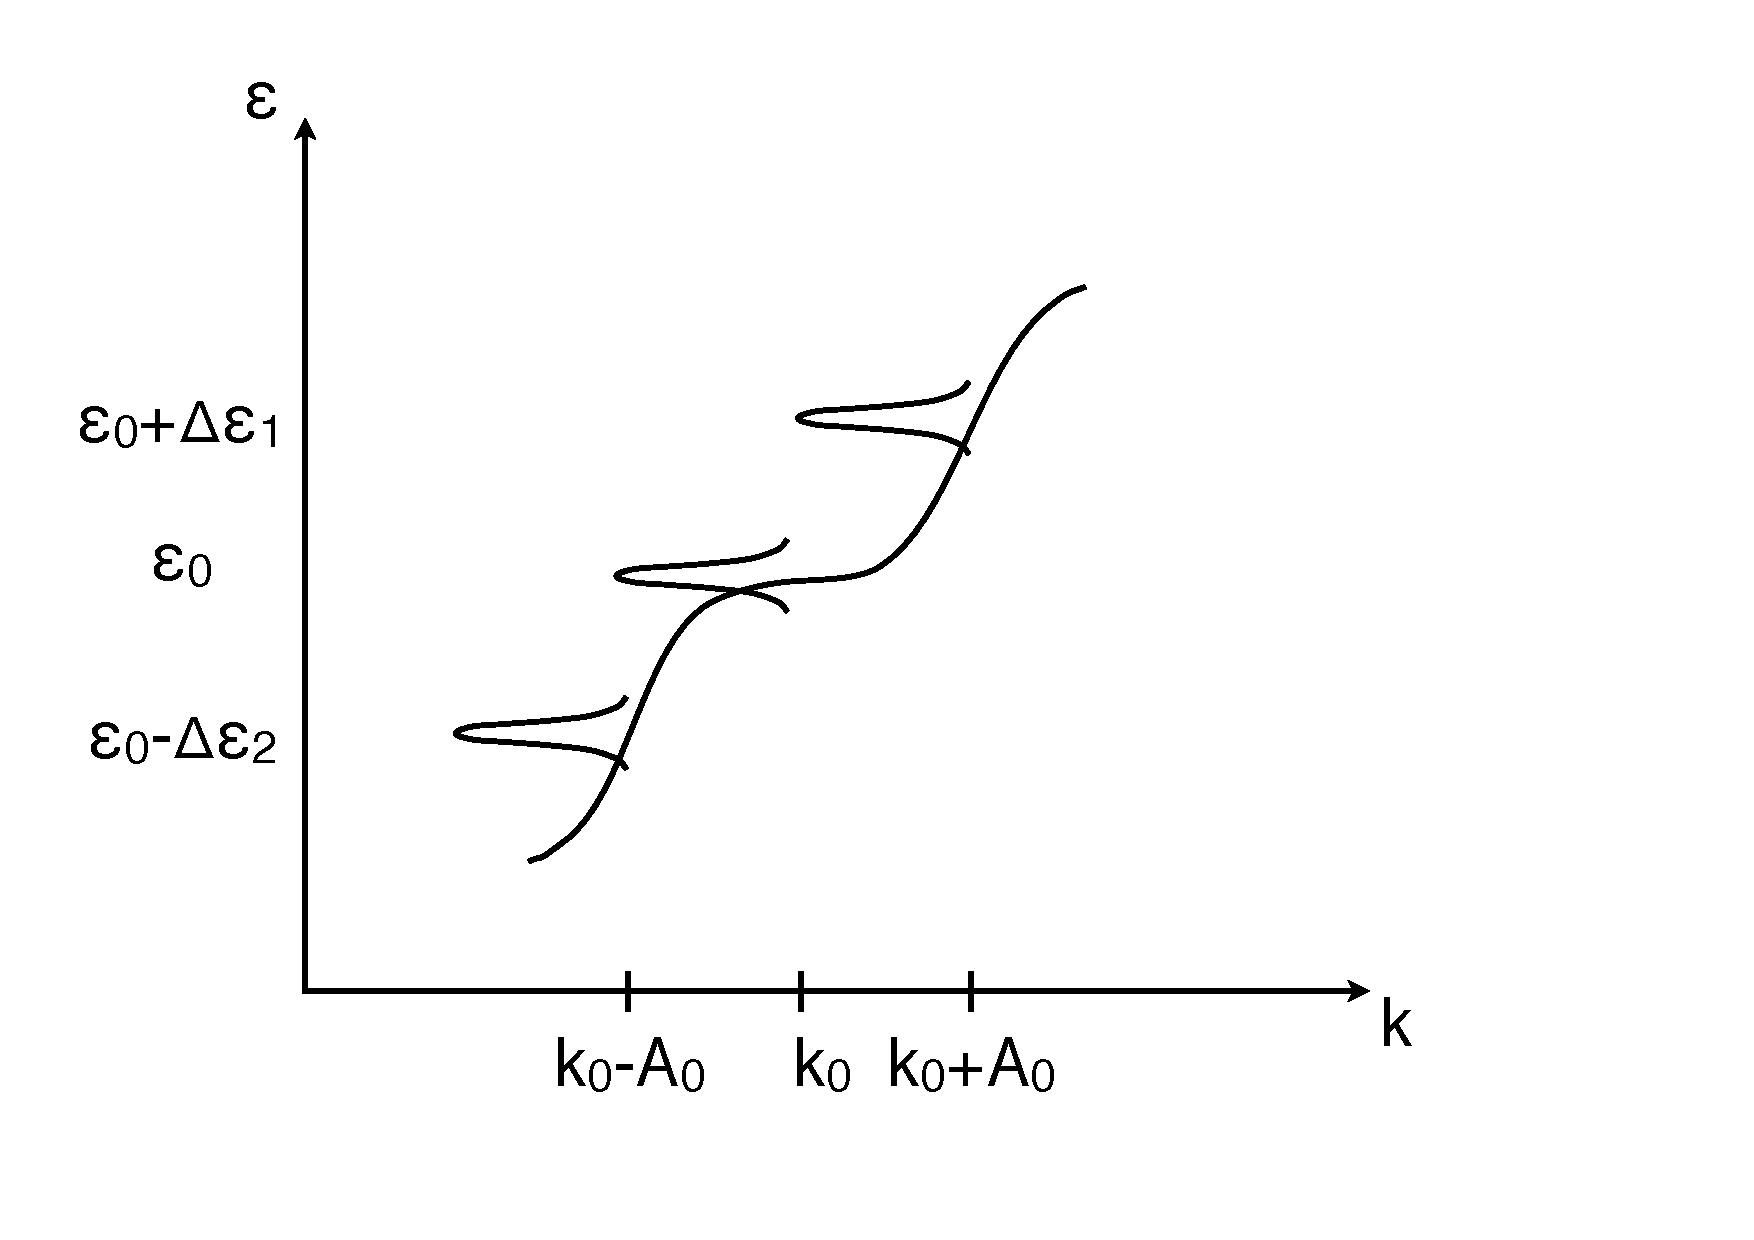
\includegraphics[width=0.5\linewidth,angle=0]{figures/Sketch1.pdf}(a)
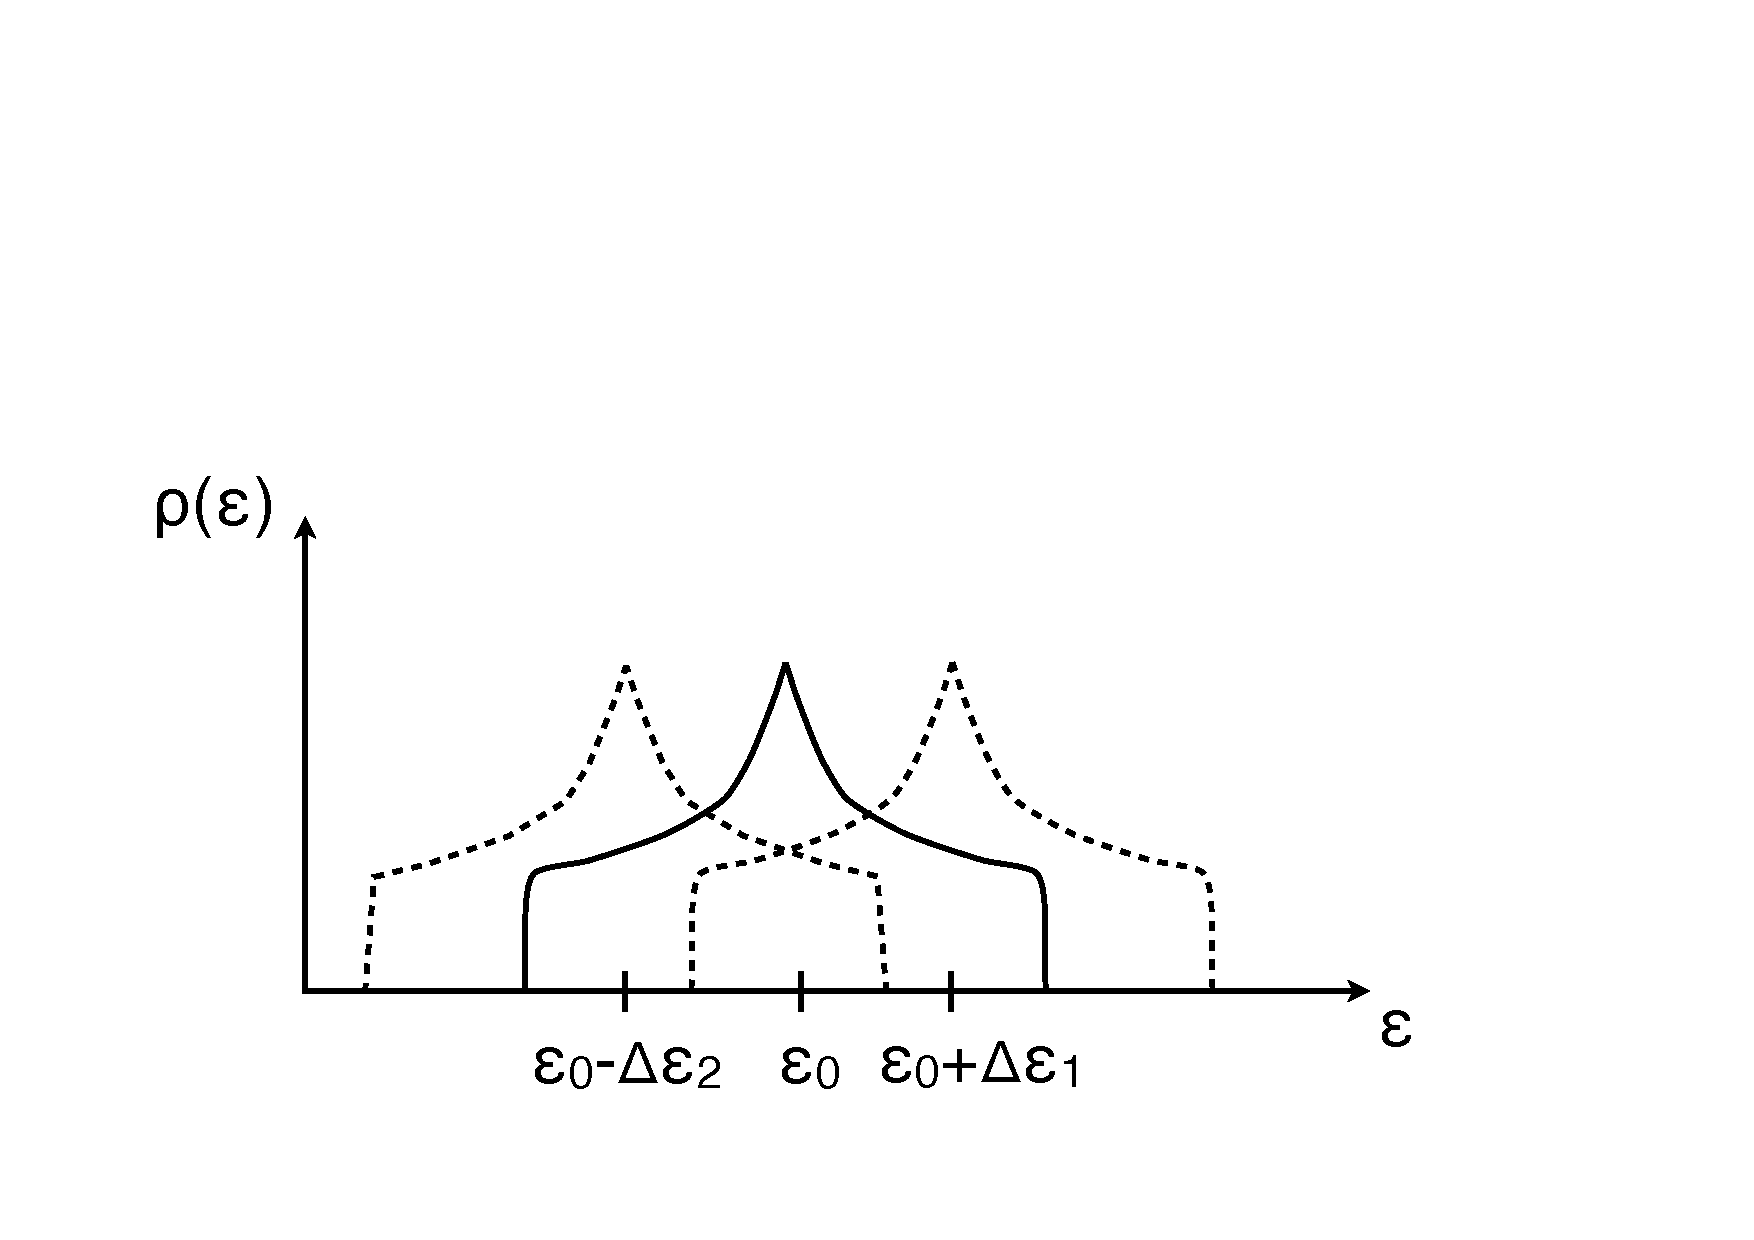
\includegraphics[width=0.5\linewidth,angle=0]{figures/Sketch2.pdf}(b)
\caption{Schematic band structure of square lattice. Pulse with vector potential amplitude $A_0$ drive the electrons with initial momentum $\bf k_0$ (zero?) from high-density region $\varepsilon_0$ to regions with momentum $\bf k_{0} \pm A_0$ and energy $\varepsilon_{0}-\Delta\varepsilon_{1}$ and $\varepsilon_{0}+\Delta\varepsilon_{2}$. 
{\color{red}{@HA I don't understand this figure AT ALL! }}
{\color{blue}{@VV Maximal intensity of Hubbard bands appears at certain values of the vector potential, namely at zeros of the zero order Bessel function ($J_0(A)$). This effect could also be called dynamical localization, because renormalizing the hoppings we increase effective Coulomb U; and at $J_0(A)=0$ we have the perfect Mott insulator.}}
}
\label{BandPulse}  
\end{figure}

%@HA you have to state the purpose of this section first, before you go into technical detail.  
%@EG added
In this section we consider behavior of the correlated system during and shortly after ultrashort pump pulse, and
analyze creation of the dynamic Mott insulating state.
%@HA how have you chosen this particualr value?
%@EG added
We choose $\lambda=3000$~nm pulse in order to maintain high enough vector potential, keep field strength reasonable for experimental applications
(low enough not to burn a sample), and fit a few-cycle pulse into calculation tilmestep window. 
%@HA what is this? 
%@EG added
We apply a short linearly polarized gaussian pulse with central frequency $\omega=0.413$~eV (wavelength $\lambda=3000$~nm), pulse duration (Full Width at half-maximum, FWHM) $d =$7.7~fs, total simulation time is 33~fs. The pulse bandwidth (FWHM) is 0.24~eV.

%We found no qualitative frequency dependence for the dynamical localization processes described in this section, at least in the range 
%$0.4\le\omega\le16$~eV. 

The peak value of the vector potential is varied in a range $A_{max} = 0.46 - 3.68$, 
that corresponds to electric fields of $5\times 10^{8} - 4\times 10^{9}$~V/m  for lattice 
constant $3.78$~\AA for $CuO_2$ plane of La cuprate. These values correspond to $0.23 - 1.8$ mJ/cm$^2$ pulse fluence for $150\times 200 \mu$m focus size.  
%@HA what do you mean by "..."?  You mean "-"?
%@EG corrected
The pulse wave vector is parallel to [001]  direction, so electric field vector is in the $CuO_2$  plane. 

{\color{red}{@HA As I have emphasized when we discussed in Hamburg, you have to 
characterize the field strength in terms of the Bessel function 
for the renormalized band width as a function of @.  
"Weak" and "strong" fields can be characterized only in terms of that.  
Then you can talk about the renormalized U/W, where W is the renormalized 
bandwidth.}}  
{\color{blue}{@EG, VV we are renormalizing the bandwidth, and the effective U is being changed in the units of renormalized bandwidth, keeping it's "bare" value constant (i.e. it is not changing w.r.t. other characteristic energies of the model, e.g. pulse frequency).}}

In this section we choose laser's linear polarization to be parallel to the lattice diagonal ([110] direction),
%$({\it xy-polarization}), 
that bring us to the situation similar to hypercube-lattice, studied e.g. in (cite !!  Tsuji et al), but here with the 2D dispersion that includes van-hove singularity and sharp band edges.  
We have also considered the case of electric field along 
one of the lattice axes ([100]).   
%({\it y-polarization}) 
Then the model becomes quasi-one-dimensional, giving results similar to ones discussed in Ref.~\cite{Rui} with no population inversion, no sign-change of the $U_{eff}$. The benchmark of our method with the exact diagonalization of a one-dimensional finite chain used in Ref.~\cite{Rui} is shown in Appendix. We also considered the case of circularly polarized short pulse, and no qualitative difference in dynamical localization processes  with respect to [110] polarization have been found.
{\color{red}{@HA Really? Hard to understand.  Anyway, you have said that 
you'll have another paper for the circularly polarized light, haven't you?}}
{\color{blue}{@VV All circularly polarized pulses are out of scope of the current paper. }}
 
The shape of the pulse vector potential is given by Eq.~\ref{Ashape} with $t_0=16.4$~fs, the profile is shown in Fig.~\ref{Pulse3A1}.  
%@HA Namely, its functional form is ***. 
%@EG done
Figure \ref{DOStdA20_25u5xyw5pi} displays the time-resolved photoemission intensity, Eq.(\ref{PES}).  
For low field strengths [Fig.\ref{DOStdA20_25u5xyw5pi}(a,b)]
 we can see the spectral weight transfers from van Hove singularity to lower Hubbard band (LHB), situated at $-U/2=-1.25$~eV. 

{\color{red}{@HA I don't understand this.  Take $t$ (nearest-neighbor hopping) as the unit of energy.  Then indicate the energy position of the vH singularity. }} 
{\color{red}{@HA As the initial state, where is the peak of the population density located?  }}
{\color{red}{@HA The color code around t (time) = 0 is no clear.  Another quite important factor is, you are dealing with the half-filled case, right?  }}
{\color{red}{@HA Then, initially, the density should be electron-hole symmetric about E=0, but this is not clear, either. }} 
%@HA You mention LHB.  Where is that located in energy?
%@EG LHB position added
{\color{blue}{@EG we changed the figures (that actually suffered from imperfectness of the Fourier transform applied, leading e.g. to particle-hole asymmetry at t=0) from population density (not used anymore) to simulated photoemission spectra (with probe FWHM = 2.5 fs)}}
 
Above a certain field strength the upper Hubbard band (UHB) starts to be populated (Fig.\ref{DOStdA20_25u5xyw5pi}(d)). At even higher fields we can see the Mott gap opening after some time, accompanied by an oscillatory behavior of the population of LHB and UHB (Fig.\ref{DOStdA20_25u5xyw5pi}(e)).


Before 6 fs the system stays metallic, 
demonstrating van Hove singularity at the Fermi energy 
% (HA)
%@whay can you say so?   Because you take V2=0 and half-filling? I don't understand the logic for saying E_F at vHsingularity makes the system metallic, either.  
%and emitting @what do you mean by "emitting?"  
%%%predominantly at the first harmonic.  !! WRONG
% (HA)
and emitting
at $\omega=0.5$ eV, see Fig. \ref{HHGw04lco8e9u25}, lower panel.
%@Are you referring to Fig. \ref{DOStdA20_25u5xyw5pi}(e)? If so, say so.  
%@ EG done.
Please note, that despite the pulse central frequency is 0.413 eV, and the current's fundamental frequency is 0.5 eV, and the third harmonic of current is at 1.5 eV (1.2 times higher).
 
Around 7 fs a gap opens due to dynamical localization.
%@HA which is due to ***?  
%@EG done.
The details of the transient processes for responses for pulses 
can be analyzed in terms of the current (Eq. \ref{Current}),
%@HA you have to give the expression for the current 
%@EG done
for high field strengths, e.g. $E_{max}=8\times 10^{9}$ V/m.
%$E_{max}=2\times 10^{10}$ V/m.  
If we plot the Gabor transform (a window Fourier transform) of the current in 
Fig. \ref{HHGw04lco8e9u25}, lower panel, we can 
see that shows dynamics of higher harmonic generation (HHG) process. 
The corresponding spectrum is shown in Fig. \ref{HHGw04lco8e9u25}, middle panel.  
{\color{red}{@HA Is the Gabor transform really meaningful for such a short 
time interval (~ 1.2 fs, which is much shorter than the 
pulse period as displayed }}
%in Fig. \ref{HHGw1p5a2e10u25}, top panel)?  
{\color{blue}{@EG the width of Gabor window was 3 fs in FWHM, actual time window is wider due to it's Gaussian nature,so it makes sense. Also, we checked ordinary FT over all time, it shows the same peak positions of current in frequency space.}}

We can then see in Fig. \ref{HHGw04lco8e9u25} that 
the HHG occurs concomitantly with the gap opening in the 
spectrum.  
Since this occurs when the field is high enough 
(for $E_{max}=8\times 10^{9}$ V/m in the present case), 
the tunneling process between Hubbard bands 
is considered to start, leading to the generation of higher harmonics.  
Around 7 fs the third harmonic starting to be generated, 
%@Do you mean $2\times, 4\times, ... \omega$ of the pulse's 
%central frequency?  If so, the side peaks seem to deviate 
%from these values.  @Why only even HHG?  
%@More seriously, how can you tell this is not an artefact ofthe Gabor transform for a shor pulse?  
%@EG corrected.

In general, as it has been checked for longer pulses, after few periods of the driving field (e.g. two periods, or 10 fs for the $\omega=0.827$~eV pulse) the double occupancy saturates to some constant value (see Fig. \ref{EtotSaturation} in Sec. \ref{Appendix2}), 
%@HA Where is the data?  You have to show them.  
%@EG added
then no more current is induced in the system, arrived at 
the dynamical Mott insulating state (cite Martin), at least for reasonable field strengths. 
%@HA Explain this!  Anyway, a gap vanishes after 15 fs in Fig. \ref{DOStdA20_25u5xyw5pi}(e), and are you referring to 
%the situation before this occurs?
%%at Amax=40 we have HHG current

The total energy and its time derivative for various pulse fluencies are shown in Fig. \ref{Etotw1p5a2e10u25}. Comparing peak values of $dE_{\rm tot}/dt$ for different pulse fluencies we can conclude (!! to Olga and Misha: $I_p$ analysis !!). Even before the phase transition to the HHG regime the maximal derivative $dE_{\rm tot}/dt$ is being reached earlier for stronger fields. @I don't see this.  For the field $2\times10^{10}$, the peak seem to appear exactly when you have the HHG.  

{\color{red}{@HA Another question is what is the physical meaning of the derivative?  }}

Some notes on $dE_{\rm tot}/dt$.  
$dE_{\rm tot}/dt|_{t=t_i}=\alpha e^{-\frac{2}{3}\frac{(2I_p)^{3/2}}{E(t_i)}}$, where $\alpha$ is unknown coefficient, $I_p$ is energy gap (and should be proportional to Hubbard U?), $E(t_i)$ is the electric field strength at time $t_i$. 
{\color{red}{@HA How have you derived this expression? }} 
Choosing the first and the second maxima of $dE_{\rm tot}/dt$ at times $t=t_1$ and $t=t_2$ we can get rid of $\alpha$ and find $I_p$.  
{\color{red}{@HA I don't understand this sentence at all.  }}
Let's note ${\dot W}_i=\left.dE_{\rm tot}/dt\right|_{t=t_i}$ and $E_i = E(t_i)$. Then $\frac{{\dot W}_1}{{\dot W}_2}=e^{-\frac{2}{3}\left(\frac{(2I_p)^{3/2}}{E_1}-\frac{(2I_p)^{3/2}}{E_2}\right)}$, and $I_p = \frac{1}{2}\left( \frac{-\frac{3}{2}ln\frac{{\dot W}_1}{{\dot W}_2}}{E_1^{-1}-E_2^{-1}} \right)^{2/3}$.  
{\color{red}{@HA So what you wanted to say with this? }}


\begin{figure}
 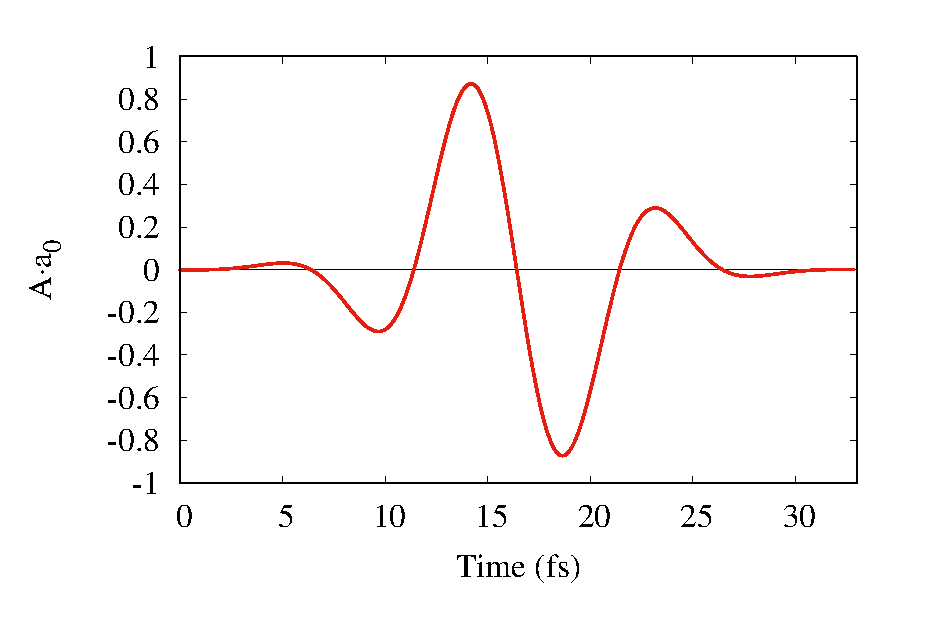
\includegraphics[width=0.5\linewidth,angle=0]{figures/Pulse3A1.eps}
\caption{Shape of the vector potential for a gaussian pulse with a central frequency $\omega=0.413$~eV, duration (FWHM) $d=7.7$~fs, and intensity $A_{max}\times a_0=1$.}
\label{Pulse3A1}  
\end{figure}

\begin{figure}
 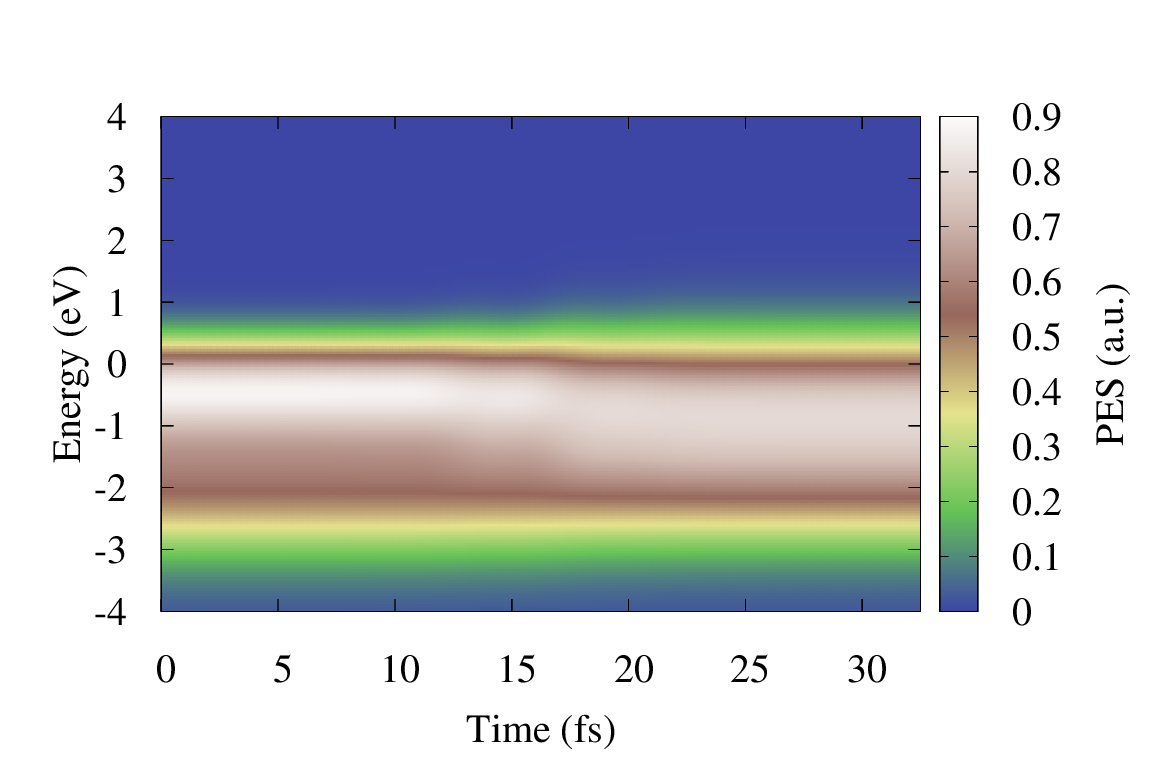
\includegraphics[width=0.5\linewidth,angle=0]{figures/3d_PES_E_5_10_8.png}(a)
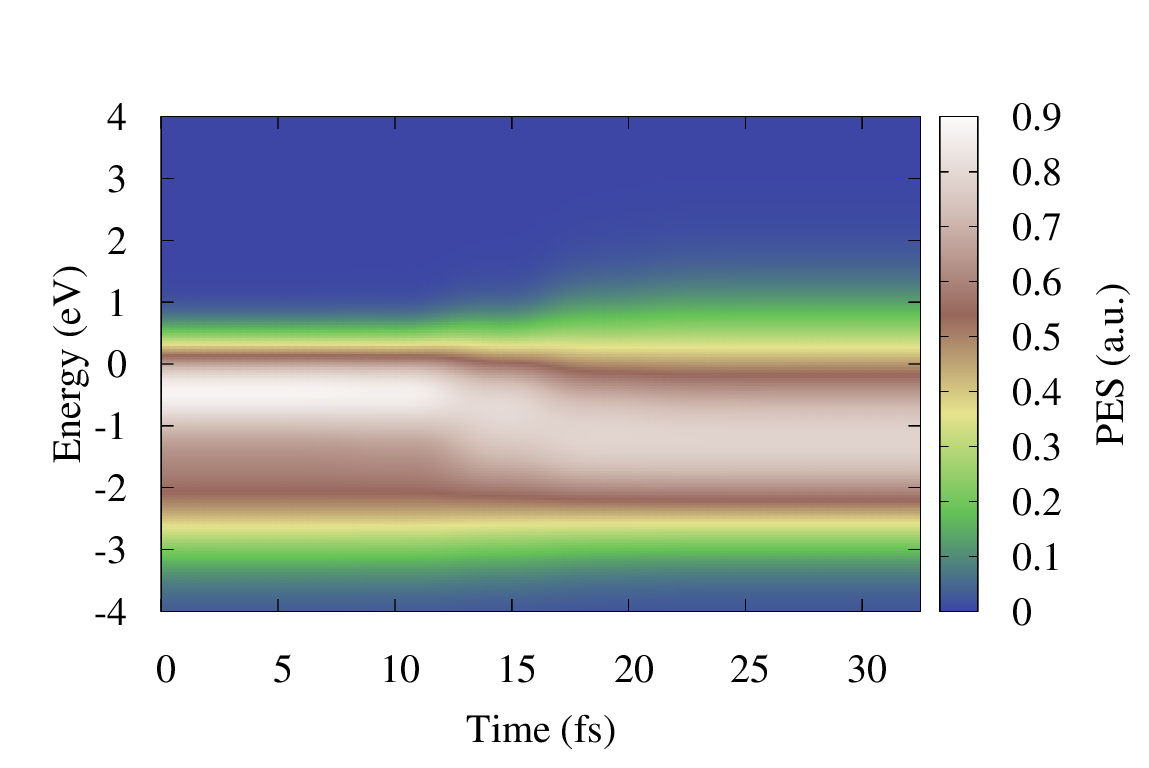
\includegraphics[width=0.5\linewidth,angle=0]{figures/3d_PES_E_8_10_8.png}(b)
 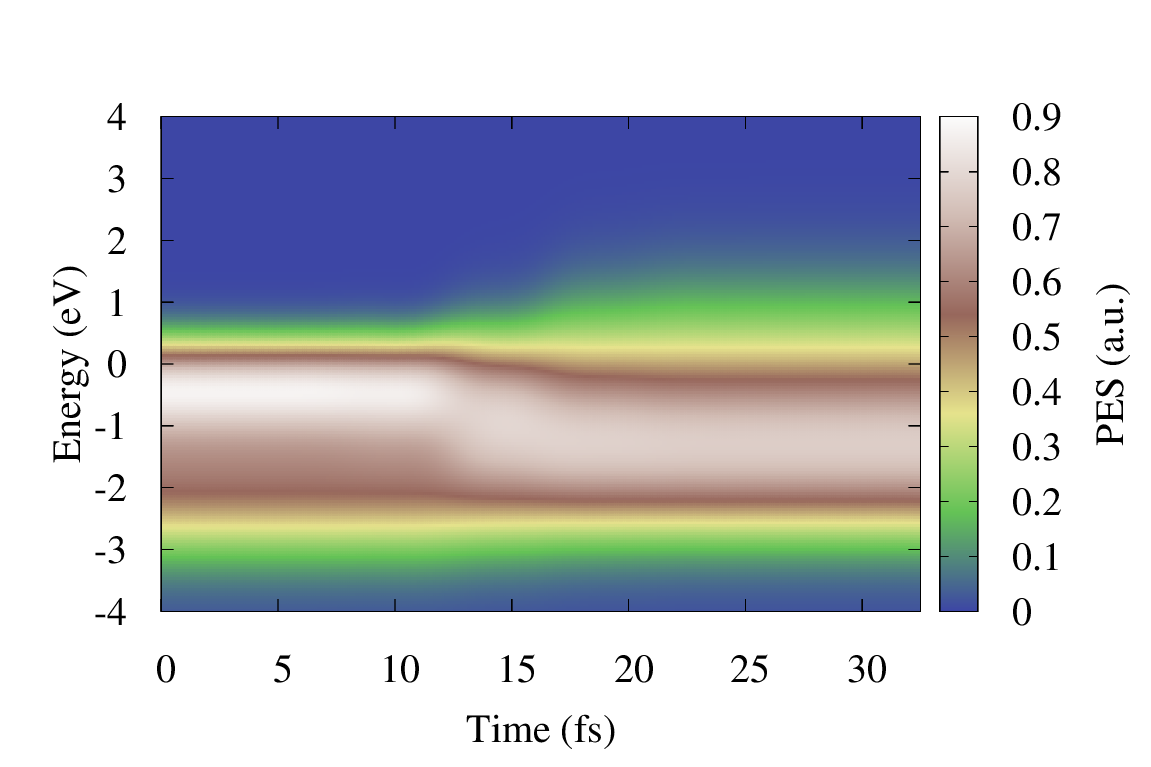
\includegraphics[width=0.5\linewidth,angle=0]{figures/3d_PES_E_1_10_9.png}(c)
 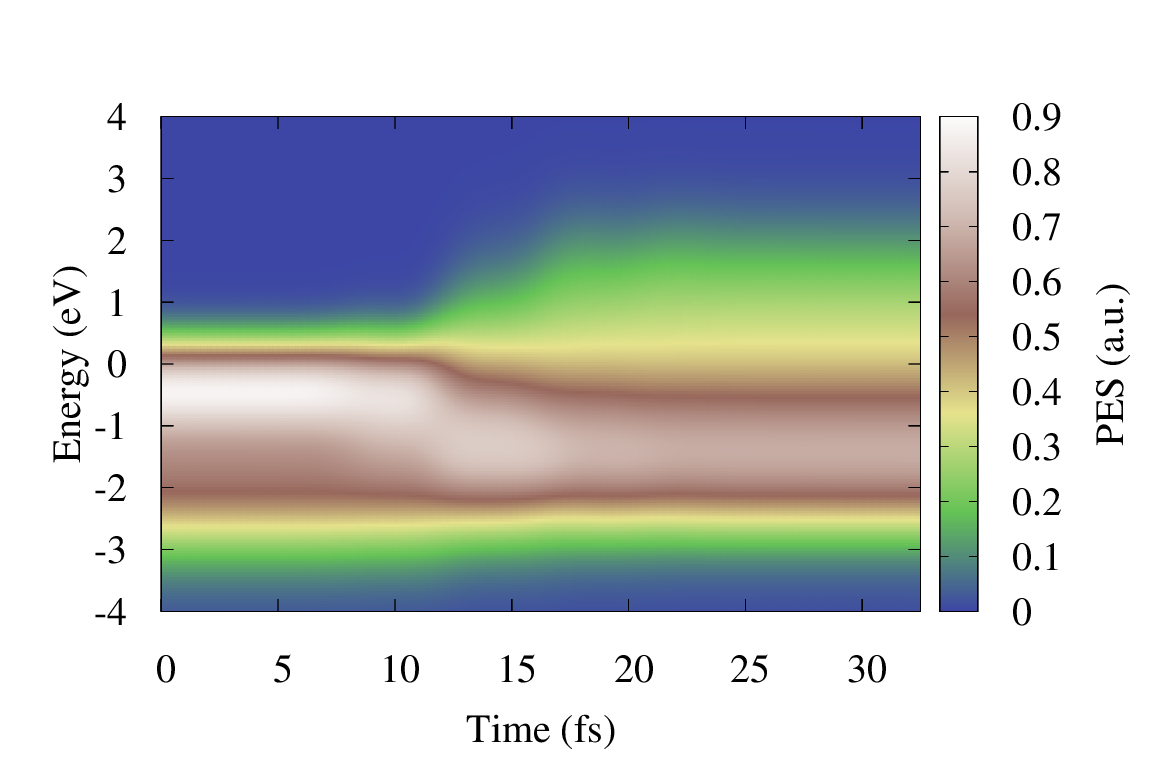
\includegraphics[width=0.5\linewidth,angle=0]{figures/3d_PES_E_2_10_9.png}(d)
 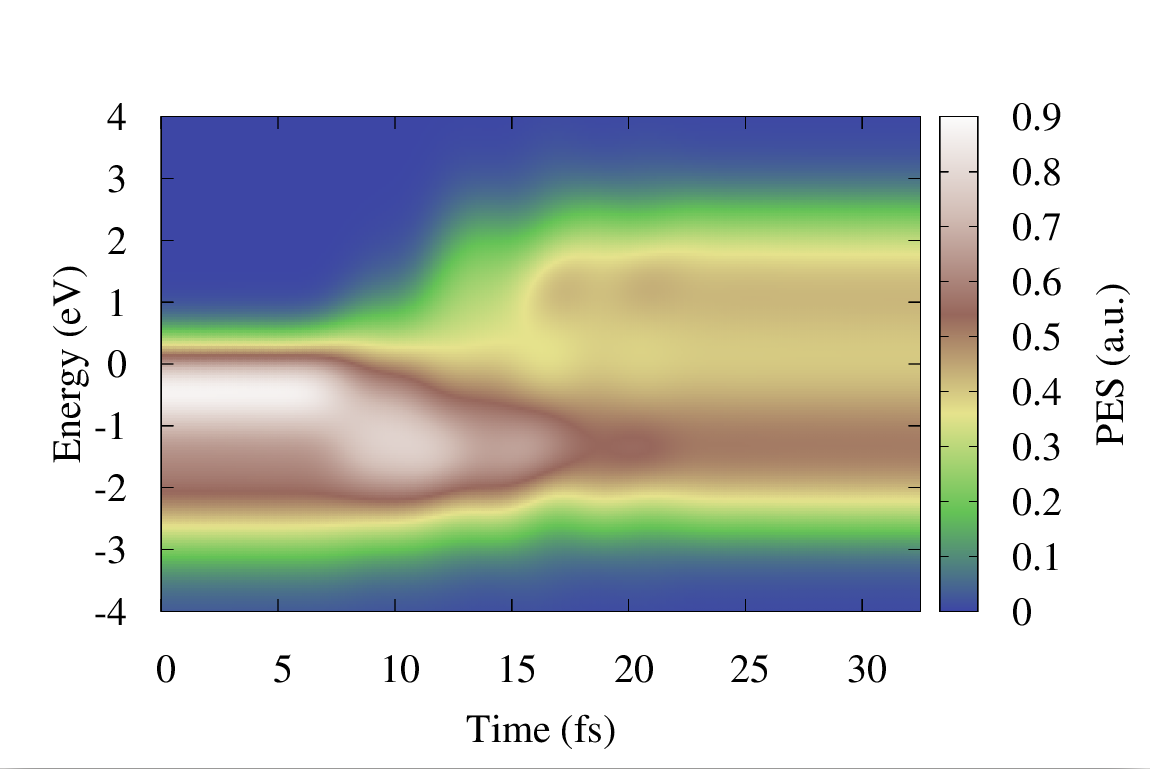
\includegraphics[width=0.5\linewidth,angle=0]{figures/3d_PES_E_5_10_9.png}(e)
\caption{Time-dependent PES for gaussian pump pulse with central frequency $\omega=0.413$~eV, $FWHM=7.7$~fs, and $E_{max}=5*10^{8}$V/m (a), $8*10^{8}$V/m (b), $1*10^{9}$V/m (c), $2*10^{9}$V/m (d), $5*10^{9}$V/m (e) with polarization along [110] direction. The probe pulse duration (FWHM) is 2.53~fs.}
\label{DOStdA20_25u5xyw5pi}  
\end{figure}


%\begin{figure}
% 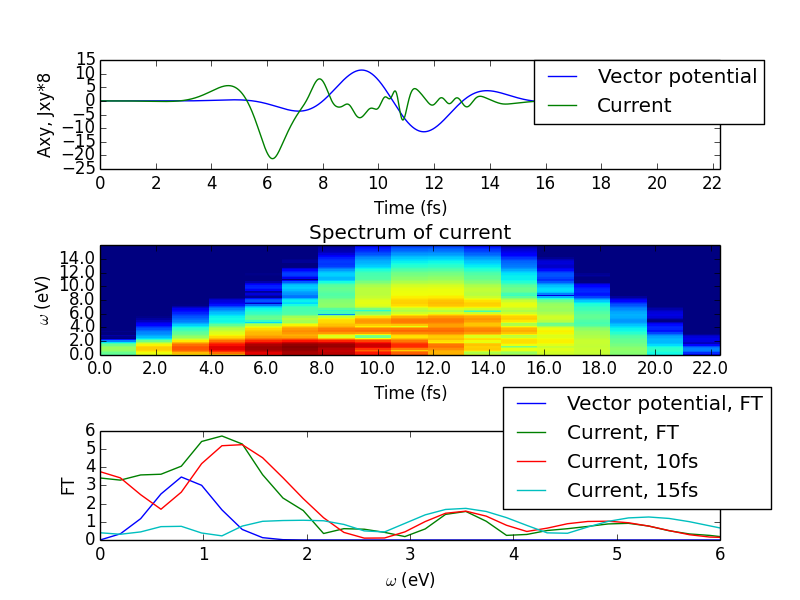
\includegraphics[width=0.7\linewidth,angle=0]{HHGw1p5a2e10u25.png}
%\caption{Upper panel: A gaussian pulse 
%(with the vector potential displayed in blue) at a central frequency $\omega=0.827$~eV, width $d=3.8$~fs, and intensity $E_{\rm max}=2\times10^{10}$~V/m, polarization along [110].  The generated current is shown in green.  Middle panel: Gabor transform of the current.  Lower panel: spectra of the incoming pulse (blue), and the current (for the @whole 
%period? in green, at 10 fs in red, 15 fs in cyan).}
%\label{HHGw1p5a2e10u25}  
%\end{figure}

\begin{figure}
 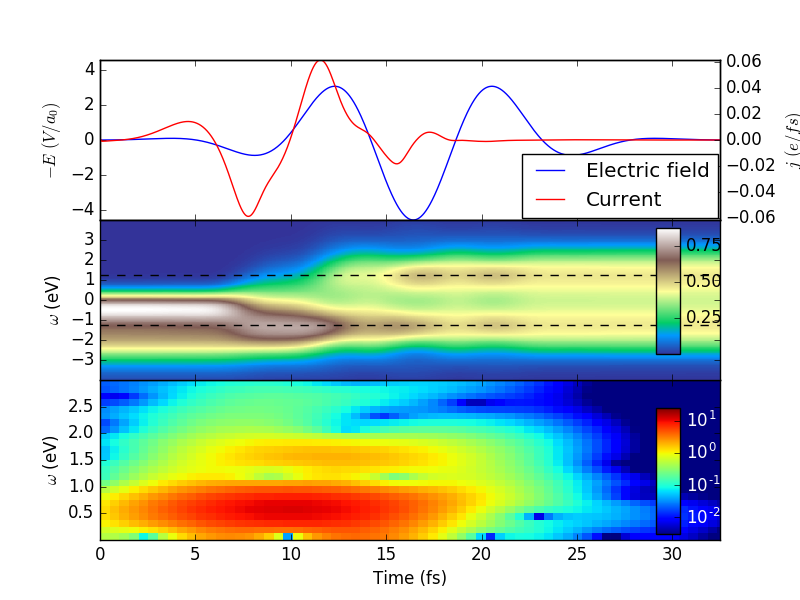
\includegraphics[width=0.5\linewidth,angle=0]{figures/HHGw04lco8e9u25.png}
\caption{Upper panel: A gaussian pulse 
(with the electric field strength displayed in blue) at a central frequency $\omega=0.413$~eV, width $d=7.7$~fs, and intensity $E_{\rm max}=8\times10^{9}$~V/m, polarization along [110].  The generated current is shown in red.  Middle panel: Time-dependent PES, dash lines denotes positions of Hubbard bands $\pm U/2$. Lower panel: Gabor transform of the current. }
\label{HHGw04lco8e9u25}  
\end{figure}

\begin{figure}
 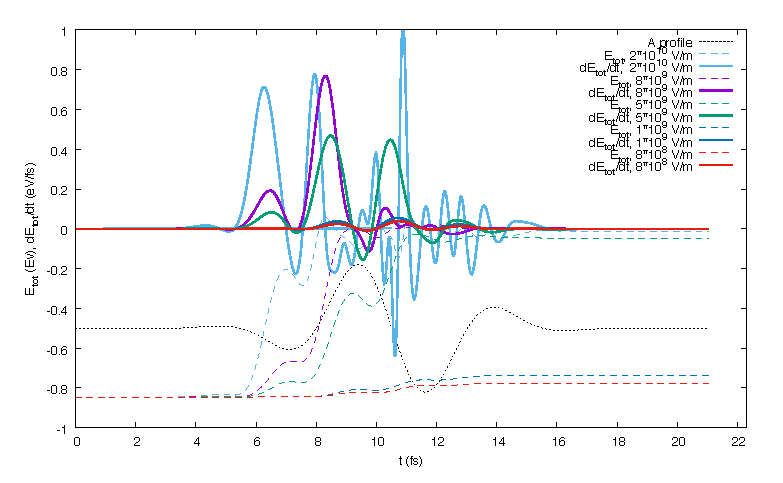
\includegraphics[width=0.5\linewidth,angle=0]{figures/Etotw1p5a2e10u25.eps}
\caption{Total energy, $E_{\rm tot}$ (dashed curves), 
and its time derivative (solid curves) for a gaussian pulse with central frequency $\omega=0.827$~eV, width $d=3.8$~fs, and 
polarization along [110] direction, for various 
intensities 
$E_{max}=8\times10^{8}, ..., 2\times10^{10}$ V/m. 
Black dotted line represents the pulse shape.}
\label{Etotw1p5a2e10u25}  
\end{figure}
\FloatBarrier



\clearpage
\bibliographystyle{abbrvnat}
\bibliography{references}
\end{document}
